
%(BEGIN_QUESTION)
% Copyright 2008, Tony R. Kuphaldt, released under the Creative Commons Attribution License (v 1.0)
% This means you may do almost anything with this work of mine, so long as you give me proper credit

Shown here is a process controller, an I/P transducer, and a loop-powered indicator:

\vskip 20pt

$$\includegraphics[width=15.5cm]{i02529x01.eps}$$

Show how the controller would connect to drive the I/P transducer and also provide a 4-20 mA DC input signal to the loop-powered indicator such that the indicator will show the percentage signal output to the I/P transducer (i.e. the approximate valve position).

\vfil 

\underbar{file i02529}
\eject
%(END_QUESTION)





%(BEGIN_ANSWER)

This is a graded question -- no answers or hints given!

%(END_ANSWER)





%(BEGIN_NOTES)

In this case, we do not need to connect anything at all to the controller's X or Y inputs -- just to the output terminals.  The controller here is acting as a ``hand'' (manual) control station, driving the I/P with a 4-20 mA current, which in turn drives the control valve with a pneumatic signal.  Since we also want the indicator to show us this valve position signal, we must connect it in series with I/P.  We know that a {\it series} circuit is necessary in order to guarantee that current will be the same through all components of the circuit.  If any parallel branches were to exist, we would have current splitting into smaller portions and therefore have some components seeing different amounts of current than others.

\vskip 10pt

This is but one valid solution to the problem.  Other solutions are possible as well:

$$\includegraphics[width=15.5cm]{i02529x02.eps}$$

\filbreak

A good problem-solving technique to apply here is sketching arrows showing where conventional flow (current) enters and exits each component, based on its voltage polarity and its identity as either a source or a load.  Once these arrows are sketched, it becomes a trivial matter to connect tip-to-tail to form a series circuit:

$$\includegraphics[width=15.5cm]{i02529x03.eps}$$

{\it Any} connections that put the tip of one arrow connecting the tail of another will form a valid series circuit!


%INDEX% Pictorial circuit review (4-20 mA loop)

%(END_NOTES)


